    
\documentclass[11pt]{article}
\usepackage[final]{graphicx}
\usepackage{times}
    \usepackage{fullpage}
    
    \title{Who's there? Occupancy prediction with smart sensor boxes.}
    \author{Jamie Sweeney - 2137284s}

    \begin{document}
    \maketitle
    



\section{Status report}

\subsection{Proposal}\label{proposal}

\subsubsection{Motivation}\label{motivation}
Room occupation detection and prediction is a quickly evolving subject of computer science and engineering, which has uses in everyday life as well as powerful industry applications. We see such detectors around us everyday, when interacting with commonplace automation such as lighting or doors, these sensors work by picking up some form of stimuli that usually becomes disrupted or augmented by human presence. With the right combination of sensors and software, it is possible to build machines that can detect, with fair accuracy, the presence or absence of human activity. Such a machine would have almost endless uses, for example automatic heating / air conditioning and lighting in office spaces, a device that could intelligently switch these function on or off depending on the situation would be greatly beneficial, compared to manual control which could result in an increased workload, as well as a financial and environmental cost.

\subsubsection{Aims}\label{aims}
The aim of this project is to design a possible 'smart sensor box' which is capable of room occupancy prediction i.e determining the amount of people in the room. Such a sensor box would typically consist of a set of sensors, which would provide the sensory input to the box, along with a micro-controller that could be used to analyse this input, either taking place on the micro-controller itself or on external hardware in combination with a central storage location \cite{ref1}.

I aim to design, implement and successfully justify the usage of such a sensor box along with any required external components. I will attempt to use the popular Raspberry Pi micro-controller, along with an array of appropriate sensors and software solutions to operate on the sensor data. The final solution should at the very least be able to determine whether a room is occupied or not, with no required estimation of the number of occupants. The optimal solution will be able to determine the occupancy with high accuracy and no range limitations, however this is unlikely to be possible with the available resources, primarily man-hours and hardware will be most limiting. The expected final solution is one that is able to predict the occupancy with high accuracy for small magnitudes, and as the magnitude of occupation increases, the accuracy will fall due to extreme collusion and higher variation of data.

\subsection{Progress}\label{progress}
\begin{itemize}
  \item Implemented very simple CPU temperature monitor, as a python function.
  \item Designed and implemented a Bluetooth scanner which can scan for nearby devices and collect addresses.
  \item Designed and implemented a Bluetooth Low Energy scanner which can scan for nearby BLE devices and collect addresses.
  \item Investigated various computer vision methods for detecting humans in an image and decided upon You Only Look Once (YOLO), specifically a type of YOLO named Tiny-YOLO was used.
  \item Integrated an existing YOLO implementation, Darknet, with a Raspberry Pi camera to allow for simple object recognition including people, at a rate of around 1 frame per 40 seconds.
  \item Upgraded to an extension of Darknet which has been optimised using NNPACK, for CPU usage, this allowed me to improve the frame rate to 1 frame per 1.5 seconds, which is a significant improvement.
  \item Set up storage buckets for external data storage on Google Storage.
  \item Designed and implemented reporter scripts for the camera detector, Bluetooth scanner and CPU temperature monitor which can maintain a state of the data while pushing all final sensor input to the Google Storage buckets for the required amount of time.
  \item Created a simple Django server that is capable of querying Google Storage for the reporter's output and using this to display a simple representation of the current state of each reported room.
\end{itemize}
\begin{figure}
  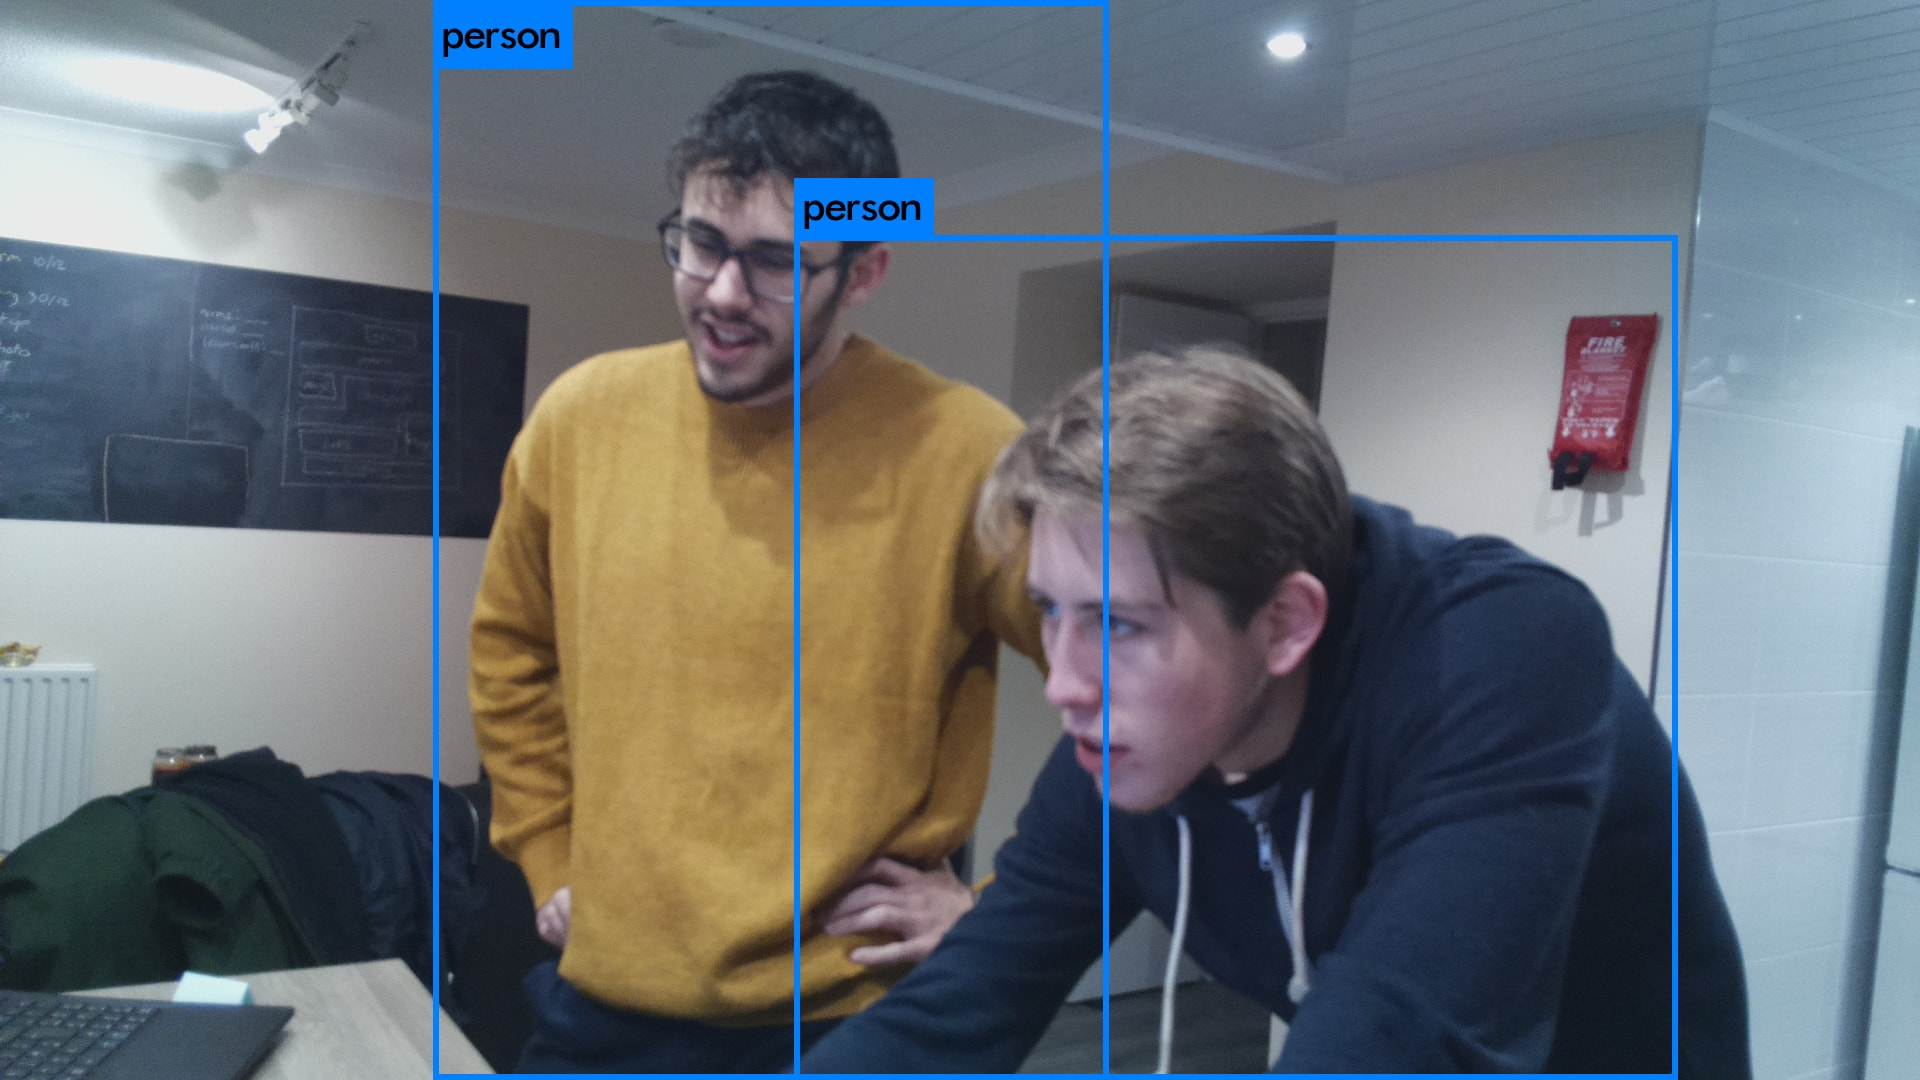
\includegraphics[scale=0.1]{yolo_example.jpg}
  \caption{Darknet image results.}
  \label{fig:result}
\end{figure}
Figure \ref{fig:result} shows an example output image for darknet with the RPi camera.

\medskip




\subsection{Problems and risks}\label{problems-and-risks}

\subsubsection{Problems}\label{problems}
There are an extremely high number of sensors available for micro-controllers such as the Raspberry Pi, for this reason it is very difficult to determine which to focus on and invest resources into. To combat this, I read as much as I could from various papers and online blog sites and tried to focus on the most commonly used sensors. In addition sensors are implemented one by one to keep plans simple and capable of modification.

Due to the low hardware capabilities of a standard micro-controller, 'in-box' object detection is very difficult and requires a lot of the available resources. At first implementation a rate of 40 seconds per frame was achieved, although this could be used somehow, it is very far from ideal, by using optimised implementations of darknet and a smaller version of YOLO we managed to obtain a much more useful rate of 1.5 seconds per frame.

\subsubsection{Risks}\label{risks}
I believe the most critical risk facing this project is the risk of balance between software solutions and sensors, in order for the sensor box to be effective, it must strike a fine balance between the sensor information that is extracted from the environment and the actual software models that are going to produce meaningful data from the sensor information. A sensor box heavily weighted in the sensors component would be able to gather a very large amount of data, but with no real method of analysis, conversely we can say that a box heavily weighted towards the software component would have great analysis potential, but not enough data to compute accurate results. Both these scenarios are highly undesirable and would be a waste of time to implement, therefore the avoid such a situation I will assess the progress of the sensor box periodically and shift my main focus as required by the balance.

Another highly possible risk is designing a system that works and is completely usable, however lacks the required documentation to roll out in bulk. Constant maintenance work and documentation of any set-up issues and requirements should be enough to allow us to prove such a product is feasible to produce in mass without much overhead costs.

\subsection{Plan}\label{plan}
\begin{itemize}
  \item 18/12 - 15/1 : Investigate possible extensions / modifications to the darknet object detection. Extend simple front-end demo a little bit. Ensure sure that mobile-data and WiFi data scanners are in fact out of scope. Perform some simple home tests and produce a set of result data that can be assessed. Investigate further sensors and techniques that could be used.
  \item 15/1 - 22/1 : Implement new sensors and obtain experimental analysis on sensor data.
  \item 22/1 - 29/1 : Investigate and undertake improvements on new features.
  \item 29/1 - 5/2 : Focus on integrating separate features and obtaining overall prediction of occupancy.
  \item 5/2 - 12/2 : Evaluation period, make concrete plans and improvements for remaining time. : Perform, document and hopefully automate the installation of the solution to a new RPi and Raspian OS image.
  \item 12/2 - 19/2 : Implement any final moderate modifications to solution. : Improve the demo Django site.
  \item 19/2 - 26/2 : Continue from previous week.
  \item 26/2 - 5/3 : Last changes to solution, final bug fixes, optimisation, clean-up and documentation.
  \item 5/3 - 12/3 : Perform final evaluation of solution, obtain result metrics and observations.
  \item 12/3 - 21/3 : Complete dissertation and finalise project.
\end{itemize}


\begin{thebibliography}{9}
\bibitem{ref1} 
Kristian Hentschel, Dejice Jacob, Jeremy Singer 
\textit{ Supersensors: Raspberry Pi Devices for Smart Campus Infrastructure}. 
Vienna, Austria, Aug. 2016.
\end{thebibliography}



\end{document}
